\section{Further Results}
\label{app:more}

\begin{figure}[t]
\centering
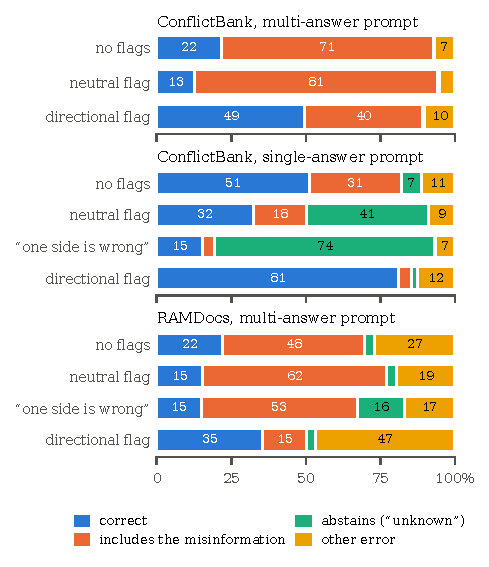
\includegraphics[width=\columnwidth]{generated/fig_answers.pdf}
\caption{What a flag does to answers on conflict questions (gpt-4o-mini, oracle pairs; share of answers, \%). The
answer policy decides how a neutral flag fails: a model told to give every valid answer adds the misinformation, and
one told there is one answer abstains. Only the directional flag raises the share of correct answers. The categories are exclusive, and an answer the primary metric scores correct counts as correct, so the misinformation share here can be a little lower than in Table~\ref{tab:risk}, which counts every answer containing a wrong answer under the bidirectional matcher.}
\label{fig:answers}
\end{figure}
\begin{table*}[t]
\centering\small
\setlength{\tabcolsep}{4pt}
\begin{tabular}{lrrrrrrrr}
\toprule
& \multicolumn{3}{c}{RAMDocs, gpt-4o-mini} & RAMDocs, gpt-4.1 & \multicolumn{3}{c}{ConflictBank, gpt-4o-mini} & \\
\cmidrule(lr){2-4}\cmidrule(lr){5-5}\cmidrule(lr){6-8}
Method & Lab. & Conflict & Clean & Lab. & All & Conflict & Clean & Calls \\
\midrule
No flags (plain), accuracy & 31.3 & 22.1 & 41.5 & 32.8 & 38.4 & 21.6 & 89.0 & 1 \\
\midrule
Instruction (v2) only & $+$2.3 & $+$5.3 & $-$1.1 & -- & $+$4.0 & $+$5.9 & $-$1.7 & 1 \\
Oracle, flag + instr. & $-$1.8 & $-$2.4 & $-$1.1 & $+$1.5 & $+$0.7 & $+$1.6 & $-$1.7 & 1 \\
Oracle, dir.\ flag + instr. & $+$6.4 & $+$13.2 & $-$1.1 & \textbf{$+$14.7} & \textbf{$+$47.4} & \textbf{$+$63.8} & $-$1.7 & 1 \\
\midrule
MADAM-RAG & $+$5.7 & $+$3.6 & $+$7.9 & -- & -- & -- & -- & 9$\times$tok. \\
Astute RAG & \textbf{$-$15.6} & $-$8.4 & \textbf{$-$23.5} & -- & \textbf{$+$18.2} & \textbf{$+$27.4} & $-$9.7 & 2 \\
Astute RAG (multi) & $-$5.9 & $-$1.2 & $-$11.1 & $+$2.3 & -- & -- & -- & 2 \\
TrustRAG & \textbf{$-$17.5} & $-$11.3 & \textbf{$-$24.3} & -- & \textbf{$+$13.9} & \textbf{$+$19.9} & $-$4.0 & 3 \\
TrustRAG (multi) & \textbf{$-$18.1} & $-$12.2 & \textbf{$-$24.6} & $-$10.9 & -- & -- & -- & 3 \\
\midrule
LLM detector, flag + instr. & $-$2.0 & $-$2.2 & $-$1.9 & -- & -- & -- & -- & 1 \\
LLM detector, dir.\ flag + instr. & $-$3.5 & $+$8.4 & \textbf{$-$16.7} & -- & -- & -- & -- & 1 \\
LLM detector, dir.\ flag & $+$4.9 & $+$12.5 & $-$3.4 & \textbf{$+$8.7} & \textbf{$+$14.8} & \textbf{$+$20.0} & $-$1.0 & 1 \\
LLM detector, remove suspect & 0.0 & \textbf{$+$18.7} & \textbf{$-$20.6} & -- & \textbf{$+$27.4} & \textbf{$+$38.8} & $-$6.7 & 1 \\
\bottomrule
\end{tabular}
\caption{Resolution instructions and published baselines. First row: accuracy (\%, one-way strict) with no flags; other rows:
paired difference from it in points. \emph{Lab.}: the labelled RAMDocs questions; ConflictBank questions are all
labelled. RAMDocs gpt-4o-mini and ConflictBank: 3 seeds; RAMDocs gpt-4.1: seed 0. \emph{instr.}: the v2 reliability
instruction. \emph{(multi)}: the baseline's final step asks for every valid answer, which RAMDocs needs (every
ConflictBank question has one answer). Calls: generator calls per question (LLM-detector rows add one detector call).
\textbf{Bold}: significant under the paper's single scheme (Section~\ref{sec:setup}).}
\label{tab:baselines}
\end{table*}

\begin{table}[t]
\centering\footnotesize
\setlength{\tabcolsep}{3pt}
\begin{tabular}{llrrrr}
\toprule
Detector & Generator & Dir.\ acc. & Gen.\ acc. & Gap & Gain \\
\midrule
gpt-6.1-terra & gpt-6.1-terra & 29.7 & 73.0 & $-$43.3 & $+$2.7 \\
gpt-6.1-terra & Claude Haiku 5.5 & 29.7 & 66.8 & $-$37.1 & \textbf{$+$4.1} \\
gpt-6.1-terra & gpt-4.1 & 29.7 & 64.7 & $-$35.0 & \textbf{$+$5.0} \\
gpt-6-luna & gpt-6.1-terra & 45.7 & 73.0 & $-$27.3 & $+$2.7 \\
gpt-6.1-terra & gpt-6-luna & 29.7 & 53.6 & $-$23.9 & \textbf{$+$7.3} \\
gpt-6-luna & Claude Haiku 5.5 & 45.7 & 66.8 & $-$21.1 & \textbf{$+$5.0} \\
gpt-6.1-terra & gpt-4o-mini & 31.3 & 51.1 & $-$19.8 & \textbf{$+$9.6} \\
gpt-6.1-terra & Qwen2.5-7B & 31.0 & 50.3 & $-$19.3 & \textbf{$+$8.0} \\
gpt-6-luna & gpt-4.1 & 45.7 & 64.7 & $-$19.0 & \textbf{$+$6.3} \\
gpt-6-luna & gpt-6-luna & 45.7 & 53.6 & $-$7.9 & \textbf{$+$11.1} \\
gpt-4o-mini & gpt-6.1-terra & 67.0 & 73.0 & $-$6.0 & \textbf{$-$11.7} \\
gpt-6-luna & gpt-4o-mini & 45.7 & 51.1 & $-$5.4 & \textbf{$+$13.7} \\
Claude Haiku 5.5 & Claude Haiku 5.5 & 61.7 & 66.8 & $-$5.1 & \textbf{$+$5.7} \\
gpt-6-luna & Qwen2.5-7B & 48.0 & 50.3 & $-$2.3 & \textbf{$+$12.0} \\
Claude Sonnet 5.5 & Claude Haiku 5.5 & 65.0 & 66.8 & $-$1.8 & \textbf{$+$8.2} \\
gpt-4o-mini & Claude Haiku 5.5 & 67.0 & 66.8 & $+$0.2 & $-$4.1 \\
gpt-4o-mini & gpt-4.1 & 67.0 & 64.7 & $+$2.3 & $-$2.3 \\
gpt-4.1 & gpt-6.1-terra & 79.0 & 73.0 & $+$6.0 & \textbf{$+$7.3} \\
Claude Haiku 5.5 & gpt-6-luna & 61.7 & 53.6 & $+$8.1 & \textbf{$+$14.3} \\
Claude Haiku 5.5 & gpt-4o-mini & 61.7 & 51.1 & $+$10.6 & \textbf{$+$13.0} \\
Claude Sonnet 5.5 & gpt-6-luna & 65.0 & 53.6 & $+$11.4 & \textbf{$+$18.1} \\
gpt-4.1 & Claude Haiku 5.5 & 79.0 & 66.8 & $+$12.2 & \textbf{$+$11.0} \\
gpt-4o-mini & gpt-6-luna & 67.0 & 53.6 & $+$13.4 & \textbf{$+$8.6} \\
Claude Sonnet 5.5 & gpt-4o-mini & 65.0 & 51.1 & $+$13.9 & \textbf{$+$15.9} \\
gpt-4.1 & gpt-4.1 & 79.0 & 64.7 & $+$14.3 & \textbf{$+$11.7} \\
gpt-4o-mini & gpt-4o-mini & 67.0 & 51.1 & $+$15.9 & \textbf{$+$8.4} \\
gpt-4o-mini & Qwen2.5-7B & 67.0 & 50.3 & $+$16.7 & \textbf{$+$7.3} \\
gpt-4.1 & gpt-6-luna & 79.0 & 53.6 & $+$25.4 & \textbf{$+$21.3} \\
gpt-4.1 & gpt-4o-mini & 79.0 & 51.1 & $+$27.9 & \textbf{$+$18.6} \\
gpt-4.1 & Qwen2.5-7B & 79.3 & 50.3 & $+$29.0 & \textbf{$+$16.0} \\
\bottomrule
\end{tabular}
\caption{Every detector--generator cell of H24 (ConflictBank, one-answer prompt, 300 conflict questions; \%).
\emph{Dir.\ acc.}: share of questions on which the detector flags the true contradiction and names its misinformation
passage; \emph{Gen.\ acc.}: the generator's accuracy with no flags; \emph{Gain}: the LLM directional flag's change in
points. Figure~\ref{fig:reliability} plots the same cells.}
\label{tab:cells}
\end{table}

\begin{table}[t]
\centering\footnotesize
\setlength{\tabcolsep}{3pt}
\resizebox{\columnwidth}{!}{%
\begin{tabular}{lr}
\toprule
\multicolumn{2}{l}{\emph{Cell level (30 cells): accuracy with the flag, $A$}} \\
$A \sim D + G$: coefficient of $D$ & 0.09 [0.03, 0.16] \\
\quad coefficient of $G$ & 0.46 [0.36, 0.55] \\
$A \sim D$ + generator FE: coefficient of $D$ & 0.09 [0.02, 0.15] \\
\quad exact permutation of $D$ across detectors & $p=0.29$ \\
\midrule
\multicolumn{2}{l}{\emph{Leave one detector out: $R^2$ for the gain}} \\
$G$ only & 0.17 \\
$D+G$ & $-$0.07 \\
gap $D-G$ (registered) & $-$0.21 \\
mechanism score & 0.62 \\
\midrule
\multicolumn{2}{l}{\emph{Question level (9000 cell-questions), points}} \\
detector right on $q$ & $+$34.5 [$+$32.8, $+$36.1] \\
detector marks a correct passage & $-$31.6 [$-$33.9, $-$29.4] \\
generator right on its own & $+$37.9 [$+$36.3, $+$39.5] \\
\midrule
\multicolumn{2}{l}{\emph{Calibration: gain $\sim$ score}} \\
slope & 0.64 [0.54, 0.74] \\
\bottomrule
\end{tabular}}

\vspace{4pt}
\begin{tabular}{lrr}
\toprule
Generator & Follows a needed & Follows a wrong- \\
& right flag & side flag \\
\midrule
Qwen2.5-7B & 61 (327) & 77 (71) \\
Claude Haiku & 57 (189) & 83 (71) \\
gpt-4.1 & 69 (171) & 83 (60) \\
gpt-4o-mini & 66 (446) & 76 (75) \\
gpt-6-luna & 75 (281) & 84 (58) \\
gpt-6.1-terra & 68 (154) & 88 (97) \\
\bottomrule
\end{tabular}
\caption{H24 without the shared $-G$ term (\S15.4, re-analysis of existing cells). $D$: the detector's direction
accuracy; $G$: the generator's no-flag accuracy. CIs: 2,000 question resamples, shared across cells. The question-level
model is a linear probability model with detector and generator fixed effects and a random intercept per question.
Lower table: share of questions the generator gets right when the detector is right and the generator alone is wrong
in every seed, and share it gets wrong when the detector marks a correct passage and the generator alone is right in
every seed (count of cell-questions in brackets).}
\label{tab:h24redo}
\end{table}

\begin{table*}[t]
\centering\footnotesize
\setlength{\tabcolsep}{4pt}
\begin{tabular}{lrlr}
\toprule
Setting & Neutral flag & Setting & Neutral flag \\
\midrule
CB forced, gpt-6.1-terra & $-$0.3 & RAMDocs, Claude Haiku & $+$1.2 \\
CB forced, gpt-4o-mini & $-$0.2 & CB one-answer, gpt-4o-mini & $-$18.7 \\
CB forced, gpt-6-luna & $+$1.6 & CB one-answer, gpt-6-luna & $-$9.4 \\
CB forced, Claude Haiku & $+$3.9 & CB one-answer, gpt-4.1 & $-$8.0 \\
CB minimal, gpt-4o-mini & $-$18.1 & CB majority, gpt-6.1-terra & $-$3.7 \\
RAMDocs, gpt-4.1 (minimal) & $-$11.0 & CB one-answer, Qwen2.5-7B & $-$3.3 \\
RAMDocs, Qwen2.5-7B (minimal) & $-$5.8 & CB one-answer, gpt-6.1-terra & $-$2.3 \\
RAMDocs, gpt-4o-mini (minimal) & $-$5.3 & RAGuard, gpt-6-luna & 0.0 \\
CB multi-answer, gpt-4o-mini & $-$8.8 & RAGuard, Claude Haiku & $+$0.3 \\
RAMDocs, gpt-4.1 (multi-answer) & $-$8.6 & CB one-answer, Claude Haiku & $+$0.7 \\
CB multi-answer, Qwen2.5-7B & $-$8.3 & CB majority, gpt-4o-mini & $+$1.1 \\
RAMDocs, gpt-4o-mini (multi-answer) & $-$6.7 & RAGuard, gpt-6.1-terra & $+$2.4 \\
CB multi-answer, gpt-4.1 & $-$6.3 & CB one-answer, Claude Sonnet & $+$3.0 \\
RAMDocs, Qwen2.5-7B (multi-answer) & $-$5.8 & RAGuard, gpt-4o-mini & $+$3.2 \\
RAMDocs, gpt-6-luna & $-$3.1 & CB majority, Claude Haiku & $+$4.3 \\
RAMDocs, gpt-6.1-terra & $-$0.7 & RAGuard, Claude Sonnet & $+$4.4 \\
RAMDocs, Claude Sonnet & 0.0 & CB majority, gpt-6-luna & $+$6.6 \\
\midrule
\multicolumn{4}{l}{\emph{Multilevel model (random effects for generator, benchmark and setting; REML)}} \\
\multicolumn{2}{l}{pooled, all settings} & \multicolumn{2}{l}{\neuMlMu\ \neuMlCI; prediction interval \neuMlPI} \\
\multicolumn{2}{l}{pooled, multi-answer prompt (10 settings)} & \multicolumn{2}{l}{$-$3.8 [$-$6.5, $-$1.0]} \\
\multicolumn{2}{l}{pooled, minimal prompt (4 settings)} & \multicolumn{2}{l}{$-$12.1 [$-$23.6, $-$0.7]} \\
\multicolumn{2}{l}{pooled, one answer prompt (16 settings)} & \multicolumn{2}{l}{$-$0.5 [$-$5.5, $+$4.5]} \\
\multicolumn{2}{l}{pooled, forced prompt (4 settings)} & \multicolumn{2}{l}{$+$1.5 [$-$1.3, $+$4.3]} \\
\midrule
\multicolumn{4}{l}{\emph{Meta-regression (same model)}} \\
\multicolumn{2}{l}{intercept (OpenAI, one answer, generated)} & \multicolumn{2}{l}{$-$2.8 [$-$8.1, $+$2.6]} \\
\multicolumn{2}{l}{several answers allowed} & \multicolumn{2}{l}{$-$3.5 [$-$8.2, $+$1.2]} \\
\multicolumn{2}{l}{forced (no unknown)} & \multicolumn{2}{l}{$+$6.4 [$+$1.6, $+$11.2]} \\
\multicolumn{2}{l}{Anthropic} & \multicolumn{2}{l}{$+$5.2 [$+$1.7, $+$8.7]} \\
\multicolumn{2}{l}{Qwen} & \multicolumn{2}{l}{$+$1.0 [$-$4.0, $+$6.0]} \\
\multicolumn{2}{l}{natural misinformation (RAGuard)} & \multicolumn{2}{l}{$+$2.7 [$-$7.0, $+$12.3]} \\
\bottomrule
\end{tabular}
\caption{The 34 settings in which the oracle neutral flag was run (conflict questions, change in
points), grouped by answer policy. The pooled estimate was registered as exploratory (\S13.4) and the multilevel model,
the policy split and the moderators in \S16.4; they use data already seen. The prediction interval describes this
design space (our generators, benchmarks and prompts), not deployments in general. \emph{Natural misinformation} is
RAGuard only; RAMDocs' misinformation is synthetic.}
\label{tab:pooled}
\end{table*}

\begin{table*}[t]
\centering\footnotesize
\setlength{\tabcolsep}{3.5pt}
\resizebox{\textwidth}{!}{%
\begin{tabular}{lrrrrrrrrr}
\toprule
& \multicolumn{4}{c}{Neutral flag, utility change at misinformation cost $c$} & Dir.\ flag & \multicolumn{4}{c}{Neutral flag: plain answer $\to$ flagged answer (null)} \\
\cmidrule(lr){2-5}\cmidrule(lr){6-6}\cmidrule(lr){7-10}
Setting & $c=0$ & $c=1$ & $c=2$ & $c=4$ & $c=2$ & mis.$\to$abst. & mis.$\to$corr. & corr.$\to$abst. & corr.$\to$mis. \\
\midrule
RAMDocs, gpt-4o-mini (multi-answer) & \textbf{$-$6.7} & \textbf{$-$20.9} & \textbf{$-$35.0} & \textbf{$-$63.3} & \textbf{$+$79.1} & 1 (0) & 2 (2) & 0 (0) & 29 (3) \\
RAMDocs, gpt-6-luna & \textbf{$-$3.1} & $-$7.7 & $-$12.2 & $-$21.3 & \textbf{$+$160.9} & 0 (0) & 1 (3) & 0 (0) & 22 (16) \\
RAMDocs, Claude Haiku & $+$1.2 & $+$9.1 & \textbf{$+$17.0} & \textbf{$+$32.9} & \textbf{$+$125.2} & 0 (0) & 9 (4) & 0 (0) & 5 (9) \\
CB multi-answer, gpt-4o-mini & \textbf{$-$8.8} & \textbf{$-$19.2} & \textbf{$-$29.7} & \textbf{$-$50.6} & \textbf{$+$91.0} & 0 (0) & 4 (3) & 1 (0) & 55 (9) \\
CB one-answer, gpt-4o-mini & \textbf{$-$18.7} & $-$5.3 & $+$8.0 & \textbf{$+$34.7} & \textbf{$+$83.7} & 45 (2) & 7 (3) & 37 (1) & 5 (2) \\
CB one-answer, gpt-6-luna & \textbf{$-$9.4} & $-$2.6 & $+$4.3 & $+$18.1 & \textbf{$+$85.1} & 27 (10) & 12 (13) & 20 (6) & 5 (6) \\
CB one-answer, gpt-6.1-terra & $-$2.3 & 0.0 & $+$2.3 & $+$7.0 & \textbf{$+$51.7} & 2 (--) & 26 (--) & 4 (--) & 5 (--) \\
CB one-answer, Claude Haiku & $+$0.7 & $+$0.6 & $+$0.4 & $+$0.2 & \textbf{$+$66.9} & 0 (0) & 25 (16) & 0 (0) & 8 (5) \\
CB one-answer, Claude Sonnet & $+$3.0 & $+$6.7 & $+$10.3 & $+$17.7 & \textbf{$+$45.7} & 2 (--) & 34 (--) & 0 (--) & 3 (--) \\
CB forced, gpt-4o-mini & $-$0.2 & $-$0.6 & $-$0.9 & $-$1.6 & \textbf{$+$74.0} & 1 (0) & 19 (4) & 0 (0) & 11 (2) \\
CB majority, gpt-4o-mini & $+$1.1 & \textbf{$+$24.6} & \textbf{$+$48.0} & \textbf{$+$94.9} & \textbf{$+$118.2} & 26 (1) & 11 (2) & 22 (1) & 8 (5) \\
RAGuard, gpt-4o-mini & $+$3.2 & $+$6.6 & $+$10.0 & $+$16.8 & \textbf{$+$34.6} & 12 (3) & 7 (3) & 8 (6) & 4 (2) \\
RAGuard, gpt-6-luna & 0.0 & $-$1.1 & $-$2.3 & $-$4.5 & \textbf{$+$29.3} & 10 (9) & 6 (9) & 8 (9) & 7 (8) \\
RAGuard, Claude Haiku & $+$0.3 & $-$1.8 & $-$4.0 & $-$8.3 & \textbf{$+$26.5} & 7 (6) & 4 (4) & 11 (9) & 6 (3) \\
\bottomrule
\end{tabular}}
\caption{Abstention-aware view of the oracle flags (conflict questions; \S15.4 and \S16.4, re-analyses of data already
seen). Utility per answer: $+1$ correct, $-c$ if it contains the misinformation, 0 for abstaining or any other wrong
answer; $c=0$ is strict accuracy. Bold: significant in one Holm family per $c$ over all \nUtilSixSettings\ settings of
Table~\ref{tab:pooled} (a selection is shown). Right: of the question--seed pairs whose plain answer contained the
misinformation (or was correct), the share whose flagged answer abstained, was correct or contained the misinformation;
in brackets the same share between two plain runs with different seeds, the churn with no flag.}
\label{tab:utility}
\end{table*}


\subsection{Where the directional flag fails (exploratory)}
\label{app:single}
After seeing the minimal-skeleton run, we split conflict questions by the number of gold answers. \nConfMulti\ of
\the\numexpr\nConfMulti+\nConfSingle\relax\ have several (same-name ambiguity \emph{and} misinformation), and a strict
answer must list all of them. On the \nConfSingle\ single-answer conflict questions, the directional flag's estimate
is positive in every setting, from \yQwenSingleOracleDir\ points (Qwen) to \yMiniSingleOracleDir\ (gpt-4o-mini), both
with the default skeleton. On multi-answer questions it changes little except with gpt-4.1 (gpt-4o-mini
\yMiniMultiOracleDir, and \yMiniMinMultiOracleDir\ with the minimal skeleton; gpt-4.1 \yFourMultiOracleDir). One reading, which
we did not test, is that a warning about one passage makes the smaller models more conservative about the legitimate
alternative answers too. Removal, which does not depend on the model acting on a warning, gains in both groups.

\subsection{Real detectors}
CAAG flags \cleanFprCaag\% of clean questions. Its neutral flags do not beat random flags at the same rate (H5;
\dCaagFlagAll\ vs.\ \dRandFlagAll\ points overall). The 90\% CI of the difference, [\tostLo, \tostHi], rules out a
gain larger than \tostHi\ points but does not establish equivalence within $\pm$\tostMargin\ points (TOST). The
addendum registered the directional-versus-neutral comparison with the LLM detector's pairs as exploratory.
Under the bidirectional metric, the LLM detector's directional flag costs clean questions \arLlmDirClean\ points. With
gpt-4.1 as the generator, its gain over all 300 questions (\gptLlmDirAll) is significant after Holm, but the 35
unlabelled questions contribute disproportionately to it (they gain \agptexclLlmDir\ points). Over the labelled
questions it is \gptlabLlmDir\ \gptlabLlmDirCI. On ConflictBank the NLI cross-encoder flags no pair:
the benchmark's passages are long, LLM-written and agree on everything but the one fact, and the truncated pair rarely
contains it.

\paragraph{Stronger models abstain in the single call.} Asked to name suspect passages before answering, the reasoning
models and Claude Haiku distrust most of ConflictBank's generated passages and abstain, losing up to
\azSgTerraSelfIdentifyClean\ points on clean questions (Table~\ref{tab:baselines}).

\paragraph{Reasoning models on RAMDocs.} With no flags, gpt-6-luna and gpt-6.1-terra are
strictly correct on few RAMDocs conflict questions because the default prompt asks for every valid answer. They give
\mixRdLunaNAnswers\ and \mixRdTerraNAnswers\ answers on average and recover \mixRdLunaRecall\% and
\mixRdTerraRecall\% of the gold answers, but \mixRdLunaMisinfo\% and \mixRdTerraMisinfo\% of their answers include
the misinformation.

\paragraph{Detector parsing.} The LLM detectors' JSON failed to parse on \parseFailTotal\ of \parseFailN\ ConflictBank
questions (a Claude Sonnet output), which then count as flagging nothing.

\subsection{A detector from another family}
Replacing the gpt-4o-mini detector with Qwen2.5-7B (gpt-4o-mini still generates) gives a much less selective
detector. It flags \qdetFpr\% of clean RAMDocs questions, but its direction accuracy is \qdetDir\%. Its directional
flag gains \zQDetLlmDirFlagDirectionalConflict\ points on conflict questions and \zQDetLlmDirFlagDirectionalClean\ on
clean ones, and its neutral flag \zQDetLlmDirFlagConflict. Removal again trades a conflict-question gain
(\zQDetLlmDirRemoveSuspectConflict) for a clean-question loss (\zQDetLlmDirRemoveSuspectClean). The conclusions do
not depend on the detector's family.

\subsection{CONFLICTS}
On the 237 automatically scorable CONFLICTS questions (exploratory, 3 seeds; most have no conflict), no condition
moves accuracy significantly (Table~\ref{tab:conflicts}).

\section{Semantic Re-score, Label Audits and Selection}
\label{app:semantic}
\begin{table*}[t]
\centering\scriptsize
\setlength{\tabcolsep}{4pt}
\begin{tabular}{llrrr}
\toprule
Setting & Contrast & Matcher (points) & Judge (points) & Judge $-$ matcher \\
\midrule
RAMDocs, gpt-4o-mini & neutral flag vs plain & $-$4.2 [$-$9.2, 0.0] & $-$2.5 [$-$9.2, $+$4.2] & $+$1.7 [$-$3.3, $+$6.7] \\
ConflictBank, gpt-4o-mini & neutral flag vs plain & $-$20.0 [$-$27.5, $-$12.5] & $-$21.7 [$-$29.2, $-$14.2] & $-$1.7 [$-$4.2, 0.0] \\
ConflictBank, Claude Haiku & neutral flag vs plain & $+$3.3 [$-$3.3, $+$10.0] & $+$6.7 [$+$0.8, $+$13.3] & $+$3.3 [0.0, $+$7.5] \\
RAMDocs, gpt-4o-mini & oracle directional flag vs answer key & $-$0.8 [$-$5.8, $+$4.2] & $+$0.8 [$-$8.3, $+$10.0] & $+$1.7 [$-$6.7, $+$10.0] \\
ConflictBank, gpt-4o-mini & oracle directional flag vs answer key & $+$10.8 [$+$4.2, $+$17.5] & $+$12.5 [$+$6.7, $+$19.2] & $+$1.7 [$-$1.7, $+$5.0] \\
ConflictBank, gpt-6-luna & oracle directional flag vs answer key & $-$1.7 [$-$5.8, $+$2.5] & 0.0 [$-$3.3, $+$3.3] & $+$1.7 [$-$1.7, $+$5.0] \\
ConflictBank, gpt-4o-mini & LLM directional flag vs verdict key & $+$3.3 [$-$2.5, $+$9.2] & $+$6.7 [$+$0.8, $+$12.5] & $+$3.3 [0.0, $+$7.5] \\
ConflictBank, gpt-6-luna & LLM directional flag vs verdict key & $-$0.8 [$-$3.3, $+$1.7] & 0.0 [$-$2.5, $+$2.5] & $+$0.8 [$-$1.7, $+$4.2] \\
ConflictBank, gpt-4o-mini & randomised directional flag vs plain & $+$4.2 [$-$5.8, $+$15.0] & $+$6.7 [$-$3.3, $+$16.7] & $+$2.5 [0.0, $+$5.8] \\
ConflictBank, Claude Haiku & randomised directional flag vs plain & $-$7.5 [$-$18.3, $+$3.3] & $-$6.7 [$-$17.5, $+$4.2] & $+$0.8 [$-$1.7, $+$3.3] \\
\bottomrule
\end{tabular}

\vspace{4pt}
\begin{tabular}{lrrrrr}
\toprule
Condition & Outputs & Matcher (\%) & Judge (\%) & Judge only (\%) & Matcher only (\%) \\
\midrule
answer key & 360 & 67.8 & 77.8 & 10.3 & 0.3 \\
directional flag (LLM) & 240 & 59.6 & 62.5 & 3.8 & 0.8 \\
directional flag (oracle) & 360 & 70.6 & 82.2 & 11.7 & 0.0 \\
neutral flag (oracle) & 360 & 36.9 & 43.3 & 6.9 & 0.6 \\
no flag & 600 & 48.8 & 53.3 & 5.2 & 0.7 \\
randomised direction (H31) & 240 & 54.6 & 59.6 & 5.0 & 0.0 \\
verdict key (LLM) & 240 & 58.3 & 59.2 & 2.1 & 1.2 \\
\bottomrule
\end{tabular}
\caption{Semantic re-score (\S17.3; exploratory). An outside-family judge (gemini-3.5-flash-lite, temperature 0) reads
the question, the reference and known wrong answers and the response, and classifies the final answer; judge-strict
means it gives the reference answer, asserts no wrong one and does not abstain. Top: each contrast on the same
120 conflict questions (seed 0) under the matcher and the judge, and their difference, with question-bootstrap
95\% CIs. Bottom: per condition, the share scored correct by each and the shares where only one does. The judge is
an LLM given the answer keys: it checks the matcher's semantics, not the benchmark labels.}
\label{tab:semantic}
\end{table*}

\paragraph{An outside-family judge changes no contrast's sign (\S17.3).} The primary metric matches answer strings. To
check whether its errors differ by condition, an LLM from a family none of our generators belongs to re-scored both
arms of \semK\ contrasts on the same \semNq\ conflict questions each (gemini-3.5-flash-lite; Table~\ref{tab:semantic}).
\S17.3 named Gemini 2.5 Flash, which was closed to new users. Judge and matcher agree on \semAgree\% of \semN\ outputs. Almost all
disagreements are answers the judge accepts and the matcher rejects (aliases, paraphrases, partial forms), and they
are condition-dependent: \semJudgeOnlyKey\% of answer-key outputs and \semJudgeOnlyDir\% of oracle-directional ones,
against \semJudgeOnlyPlain\% without a flag. The failure we were most concerned about, a final answer such as
``$Y$, not $X$'' counted as asserting the wrong answer $X$, occurs in \semRejected\% of outputs. Because
both arms of each contrast gain, the judge moves every contrast by \semDidMin\ to \semDidMax\ points. No conclusion
changes sign, and the matcher-scored differences are slightly conservative. With \semNq\ questions per contrast these
intervals are too wide to confirm the $\pm$3-point equivalence claims, which therefore rest on the matcher. The
judge is given the answer keys, so it tests the scorer, not the benchmark labels. A blinded, paired human-audit sheet of
150 of these pairs and 50 RAGuard post pairs is released unlabelled (\texttt{runs/labelling/audit8\_*}).

\paragraph{The WikiContradict harm holds under its original rubric.} The original evaluation counts an answer correct when it gives
both answers, acknowledges that they conflict and does not prefer one without support
\citep[\S3.4]{hou2024wikicontradict}. Judged that way, the LLM directional flag changes the share of correct answers
by \wikiOrigMiniEff\ points for gpt-4o-mini (\wikiOrigMiniPlain\% to \wikiOrigMiniDir\%), \wikiOrigLunaEff\ for
gpt-6-luna and \wikiOrigHaikuEff\ for Claude Haiku (seed 0, all 253 questions), so the H28 harm holds. For gpt-4o-mini the flag raises the share that merely mentions both answers (\wikiBothMiniEff) while
lowering the share that acknowledges the conflict without an unsupported preference.

\paragraph{RAGuard pairs rarely contradict.} RAGuard labels a post supporting or misleading by whether GPT-4 judged the claim correctly
with it in context, so its ``contradiction pairs'' are a transfer of behavioural labels. Of \rgAudN\ sampled
supporting~$\times$~misleading pairs, the judge finds that the two posts cannot both be right about the claim in
\rgAudContradict\%. It finds the misleading post false about the claim in \rgAudBFalse\% (unclear in
\rgAudBUnclear\%) and the supporting post consistent with the verdict in \rgAudASupports\%. All three hold for
\rgAudVerified\%. Most pairs discuss the claim from different angles rather than assert opposite
facts. RAGuard's oracle-flag rows therefore test what a generator does with these labels, not with verified
contradictions, and we draw no factual-oracle conclusion from them. This audit uses one LLM judge; the released
human sheet covers 50 of these pairs.

\begin{table*}[t]
\centering\scriptsize
\setlength{\tabcolsep}{3pt}
\begin{tabular}{llrrrrrrrrrrrr}
\toprule
& & & & \multicolumn{3}{c}{Flag names the false side} & \multicolumn{3}{c}{Flag marks a correct passage} & Rest & \multicolumn{3}{c}{Gain (points)} \\
\cmidrule(lr){5-7}\cmidrule(lr){8-10}\cmidrule(lr){12-14}
Generator & Detector & Prec. & Rec. & Share & Acc. & Gain & Share & Acc. & Gain & contrib. & Marginal & Question & Observed \\
\midrule
gpt-4o-mini & Claude Haiku & 78 & 79 & 62 & 58 & $+$28.8 & 11 & 42 & $-$30.4 & $-$1.3 & $+$16.1 & $+$12.3 & $+$13.0 \\
gpt-4o-mini & Claude Sonnet & 78 & 84 & 65 & 51 & $+$32.8 & 10 & 40 & $-$20.7 & $-$3.4 & $+$15.8 & $+$16.1 & $+$15.9 \\
gpt-4o-mini & gpt-4.1 & 82 & 97 & 79 & 55 & $+$28.6 & 8 & 25 & $-$22.2 & $-$2.2 & $+$18.3 & $+$19.2 & $+$18.6 \\
gpt-4o-mini & gpt-4o-mini & 69 & 97 & 67 & 60 & $+$23.1 & 30 & 30 & $-$23.1 & 0.0 & $+$10.5 & $+$10.4 & $+$8.4 \\
gpt-4o-mini & gpt-6-luna & 82 & 56 & 46 & 50 & $+$36.7 & 7 & 57 & $-$46.7 & 0.0 & $+$18.5 & $+$11.0 & $+$13.7 \\
gpt-4o-mini & gpt-6.1-terra & 83 & 38 & 31 & 51 & $+$36.9 & 4 & 61 & $-$36.1 & $-$0.6 & $+$19.2 & $+$7.4 & $+$9.6 \\
gpt-6-luna & Claude Haiku & 78 & 79 & 62 & 61 & $+$31.5 & 11 & 45 & $-$34.3 & $-$1.2 & $+$16.3 & $+$13.5 & $+$14.3 \\
gpt-6-luna & Claude Sonnet & 78 & 84 & 65 & 59 & $+$34.5 & 10 & 41 & $-$35.6 & $-$0.9 & $+$16.0 & $+$16.2 & $+$18.1 \\
gpt-6-luna & gpt-4.1 & 82 & 97 & 79 & 60 & $+$31.1 & 8 & 21 & $-$20.8 & $-$1.6 & $+$19.2 & $+$21.6 & $+$21.3 \\
gpt-6-luna & gpt-4o-mini & 69 & 97 & 67 & 63 & $+$27.0 & 30 & 33 & $-$31.5 & 0.0 & $+$9.1 & $+$10.0 & $+$8.6 \\
gpt-6-luna & gpt-6-luna & 82 & 56 & 46 & 64 & $+$29.2 & 7 & 40 & $-$35.0 & $+$0.1 & $+$19.4 & $+$9.8 & $+$11.1 \\
gpt-6-luna & gpt-6.1-terra & 82 & 36 & 30 & 66 & $+$30.3 & 4 & 56 & $-$38.5 & 0.0 & $+$19.7 & $+$5.4 & $+$7.3 \\
Claude Haiku & Claude Haiku & 78 & 79 & 62 & 79 & $+$14.8 & 11 & 28 & $-$22.5 & $-$0.9 & $+$8.0 & $+$6.1 & $+$5.7 \\
Claude Haiku & Claude Sonnet & 78 & 84 & 65 & 74 & $+$18.1 & 10 & 53 & $-$37.9 & $+$0.1 & $+$7.8 & $+$7.3 & $+$8.2 \\
Claude Haiku & gpt-4.1 & 82 & 97 & 79 & 73 & $+$18.0 & 8 & 17 & $-$16.7 & $-$1.9 & $+$10.7 & $+$12.7 & $+$11.0 \\
Claude Haiku & gpt-4o-mini & 69 & 97 & 67 & 78 & $+$12.6 & 30 & 43 & $-$41.4 & 0.0 & $+$1.3 & $+$1.1 & $-$4.1 \\
Claude Haiku & gpt-6-luna & 82 & 56 & 46 & 78 & $+$14.8 & 7 & 45 & $-$15.0 & $-$0.8 & $+$10.9 & $+$4.4 & $+$5.0 \\
Claude Haiku & gpt-6.1-terra & 82 & 36 & 30 & 76 & $+$18.0 & 4 & 67 & $-$28.2 & 0.0 & $+$11.2 & $+$2.7 & $+$4.1 \\
gpt-6.1-terra & gpt-4.1 & 82 & 97 & 79 & 74 & $+$16.9 & 8 & 62 & $-$62.5 & $-$1.0 & $+$2.6 & $+$9.0 & $+$7.3 \\
gpt-6.1-terra & gpt-4o-mini & 69 & 97 & 67 & 79 & $+$10.4 & 30 & 62 & $-$61.5 & 0.0 & $-$8.0 & $-$8.4 & $-$11.7 \\
gpt-6.1-terra & gpt-6-luna & 82 & 56 & 46 & 77 & $+$13.1 & 7 & 80 & $-$45.0 & $-$0.3 & $+$2.9 & $+$2.1 & $+$2.7 \\
gpt-6.1-terra & gpt-6.1-terra & 82 & 36 & 30 & 80 & $+$14.6 & 4 & 77 & $-$30.8 & $-$0.3 & $+$3.2 & $+$0.8 & $+$2.7 \\
Qwen2.5-7B & gpt-4.1 & 82 & 97 & 79 & 50 & $+$27.3 & 8 & 43 & $-$39.1 & $-$2.7 & -- & $+$23.4 & $+$16.0 \\
Qwen2.5-7B & gpt-4o-mini & 69 & 97 & 67 & 54 & $+$25.9 & 30 & 44 & $-$33.0 & 0.0 & -- & $+$10.2 & $+$7.3 \\
Qwen2.5-7B & gpt-6-luna & 83 & 58 & 48 & 50 & $+$30.6 & 7 & 65 & $-$25.0 & $-$1.0 & -- & $+$12.4 & $+$12.0 \\
Qwen2.5-7B & gpt-6.1-terra & 83 & 37 & 31 & 54 & $+$25.8 & 4 & 67 & $-$16.7 & $+$0.7 & -- & $+$7.3 & $+$8.0 \\
gpt-4.1 & gpt-4.1 & 82 & 97 & 79 & 72 & $+$19.8 & 8 & 21 & $-$20.8 & $-$2.3 & -- & $+$13.2 & $+$11.7 \\
gpt-4.1 & gpt-4o-mini & 69 & 97 & 67 & 77 & $+$13.9 & 30 & 38 & $-$38.5 & 0.0 & -- & $+$1.7 & $-$2.3 \\
gpt-4.1 & gpt-6-luna & 82 & 56 & 46 & 75 & $+$18.2 & 7 & 55 & $-$35.0 & $+$0.3 & -- & $+$4.7 & $+$6.3 \\
gpt-4.1 & gpt-6.1-terra & 82 & 36 & 30 & 74 & $+$20.2 & 4 & 69 & $-$23.1 & 0.0 & -- & $+$2.8 & $+$5.0 \\
\bottomrule
\end{tabular}
\caption{The crossed cells (ConflictBank, one-answer prompt, conflict questions) split by what the flag does on each
question (exploratory, \S17.1). \emph{Prec.}, \emph{Rec.}: direction precision and recall of the gold pair (\%).
\emph{Share}: share of the cell's questions; \emph{Acc.}: the generator's no-flag accuracy on them (\%); \emph{Gain}:
the flag's mean effect on them (points). \emph{Rest}: the remaining questions' contribution to the gain.
\emph{Marginal}: the break-even calculation, $pR+(1-p)W$ with H31's $R$ and $W$ at the cell's precision $p$, which assumes
every question is flagged on its true pair and that flagged questions are typical; \emph{Question}: the follow-rate
account from each question's own flag and no-flag answer; both are retrospective. Generators without an H31 run have no
marginal prediction; their question-level prediction uses mean follow rates.}
\label{tab:selection}
\end{table*}

\paragraph{Selection in the crossed cells.} Table~\ref{tab:selection} splits each crossed cell by what the flag does
on each question. The marginal break-even calculation (precision times $R$ plus its complement times $W$, at full
coverage) has mean error \selMargMae\ points against the observed gains (\selMargCovMae\ when scaled by recall); the
follow-rate account, which uses each cell's coverage and no-flag accuracy, has \predEightMae\ \predEightMaeCI.

\section{Reproducibility}
\label{app:repro}